% Requires running Bibtex

\documentclass[%
reprint,
amsmath,amssymb,
aps,
]{revtex4-2}

\usepackage{graphicx}% Include figure files
\usepackage{dcolumn}% Align table columns on decimal point
\usepackage{bm}% bold math
\usepackage{hyperref}% add hypertext capabilities
\usepackage[font=scriptsize,labelfont=bf, justification=justified]{caption}% change fontsize in captions
\usepackage{booktabs}% cool table style
\hypersetup{
	colorlinks=true,       % false: boxed links; true: colored links
	linkcolor=black,        % color of internal links
	citecolor=black,        % color of links to bibliography
	filecolor=black,     % color of file links
	urlcolor=black         
}

\usepackage{bibspacing}
\setlength{\bibitemsep}{.5\baselineskip plus .05\baselineskip minus .05\baselineskip}


\begin{document}
	
	\preprint{APS/123-QED}
	
	\title{PHYC30170 Physics with Astronomy and Space Science Lab 1;\\Astronomical Image Analysis}% Force line breaks with \\
	
	\author{Daragh Hollman}
	\email{daragh.hollman@ucdconnect.ie}
	
	\date{\today}
	
	\begin{abstract}
		The aim of this experiment was to reduce and analyse images of the galaxy Messier 91 (M91) and the eclipsing binary system NN Serpentis (NN Ser). The aim was to determine the angular size of M91 and the plot the lightcurve of NN Ser. We calculated the apparent size of Messier 91 to be $\left(21.8 \pm 4.3\right) \,\text{kpc}$ $\times$ $\left(20.7 \pm 4.5\right) \,\text{kpc}$. Adjusting for a position angle of $150^\circ$ and an inclination of $36.9^\circ$, the physical size of the galaxy was calculated to be $\left(54 \pm 11\right) \,\text{kpc}$ $\times$ $\left(51 \pm 11\right) \,\text{kpc}$. The lightcurve of NN Ser was also determined and plotted plotted, and the duration of the eclipse was determined to be $(11.1 \pm 1.2)\,\text{minutes}$. From this light curve, a lower limit on the ratio of the masses of the stars in NN Ser was calculated to be $0.7 \pm 0.3$.
	\end{abstract}

	\maketitle
	
	\section{Introduction}

		Astronomical image analysis is fundamental to the understanding of celestial objects and the physical processes behind them. It involves many techniques to determine the properties of such celestial objects including image reduction and aperture photometry, both of which are explored in this report.
	
	
	\section{Theory}
		\subsection{Image Reduction}
			When taking images in astronomy there exists a level of background noise and non-uniformities which must be accounted for to ensure accurate measurements. Removing these effects is known as data reduction\cite{manual}. This noise comes from many things including readout electronics, thermal emissions, and non-uniformities in the detector\cite{astropy}. To ameliorate some of these noises and remove non-uniformities, flat field and bias frames are taken. Flat field frames (flats) are controlled, uniformly illuminated images used to correct for non-uniformities in the detector. Any defects in the detector would appear non uniform in these images which can be used to map the sensitivity variations across the image\cite{olivier}. Bias frames (biases) are images taken with a near (ideally exactly) zero second exposure time. These are used to counteract a constant background that is present in all images. They contain no light and hence provide a offset which can be subtracted from all further images. Unwanted signals due to thermal emissions known as dark current can be accounted for by keeping the imaging device cool.
		
		\subsection{Size Calculations}
		
			\subsubsection{Angular and Apparent Size}
			
					\begin{figure}
						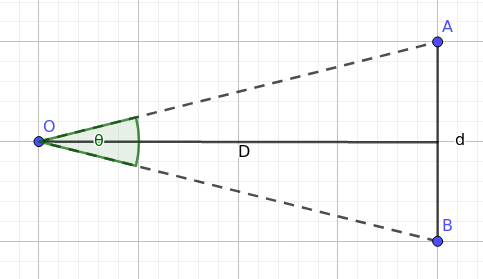
\includegraphics[width=0.75\columnwidth]{apparentSize.png}
						\caption{\label{fig:trig} A diagram showing the construction of the angular size $\theta$ in equation \ref{eq:arctan}. Line $d$ is the apparent size of the galaxy and $D$ is the distance to it. Figure made using GeoGebra.}
					\end{figure}
					
					To find the physical size of the galaxy the angular size first needs to be calculated. The angular size of the source can be determined using trigonometry using equation \ref{eq:arctan} which is constructed in figure \ref{fig:trig}.
					\begin{equation}
						\theta = 2 \arctan{\left(\frac{d}{2 D}\right)}
						\label{eq:arctan}
					\end{equation}Here, $\theta$ is the angular size, $d$ is the apparent size and $D$ is the distance between the source and the observer. This equation can be rearranged to get an expression for the apparent size using the small angle approximation to create equation \ref{eq:angSize}.
					\begin{equation}
						d = \frac{\theta}{206265\,\text{arcsec}} D
						\label{eq:angSize}
					\end{equation}The divisor is introduced to be able to work with $\theta$ in units of arcseconds as there are approximately $206,265$ arcseconds in a radian\cite{modernAstro}.
				
		
			\subsubsection{\label{sec:paAndI}Adjusting for Position Angle and Inclination}
				To convert from an apparent size to a physical size some adjustments need to be made to account for both the position angle and the inclination of the galaxy. Position angle is the angle on the celestial sphere which moves from north to south eastwards whereas inclination is the angle of orientation of the plane of the source relative to the plane of the observer. Figure \ref{fig:positionAngle} shows how the position angle can be accounted for using the trigonometric rule that corresponding angles are congruent between parallel lines. The adjustment made on the observed diameter is given by equation \ref{eq:positionAngle}:
				
				\begin{equation}
					d_\text{adjusted} = \frac{d_\text{observed}}{\sin{\left(\pi - \phi\right)}}
					\label{eq:positionAngle}
				\end{equation}where $\phi$ is the position angle and $d$ is the apparent size of the source. Figure \ref{fig:inclination} shows how the inclination of the source with respect to the plane of the observer can be accounted for using the trigonometric functions. This is described in equation \ref{eq:inclination}:
			
				\begin{equation}
					d_\text{adjusted} = \frac{d_\text{observed}}{\cos{\left(i\right)}}
					\label{eq:inclination}
				\end{equation}where $i$ is the inclination of the galaxy with respect to the plane of the observer. Combining both the adjustment due to position angle and the adjustment due to inclination yields the final adjustment factor describe in equation \ref{eq:adj}.
			
				\begin{equation}
					d_\text{adjusted} = \frac{d_\text{observed}}{\cos{\left(i\right)}\sin{\left(\pi - \phi\right)}}
					\label{eq:adj}
				\end{equation}
			
				\begin{figure}
					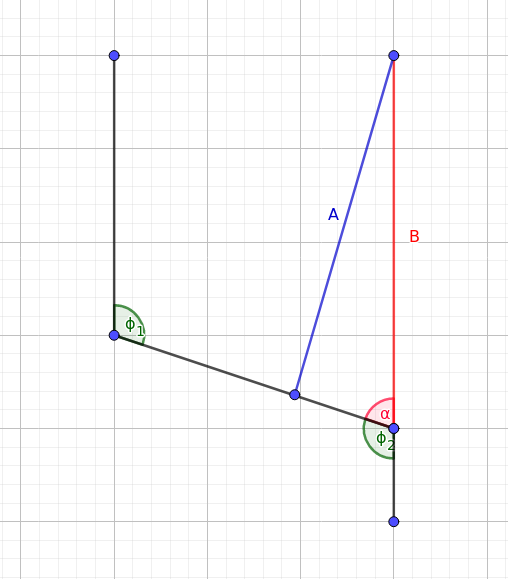
\includegraphics[width=0.75\columnwidth]{positionAngle.png}
					\caption{\label{fig:positionAngle} A diagram of how the position angle can be accounted for. The actual size of the source is marked by line B whereas the apparent size is marked by line A. We can solve for $\alpha$ in terms of the position angle using the law that corresponding angles are congruent for parallel lines. Figure made using GeoGebra.}
				\end{figure}
			
				\begin{figure}
					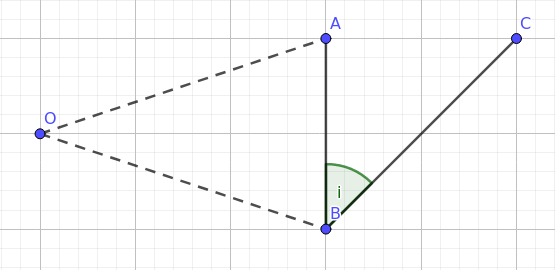
\includegraphics[width=0.75\columnwidth]{inclinationAdjustment.png}
					\caption{\label{fig:inclination} A diagram of how the inclination is accounted for. The observer at O sees the galaxy as line segment AB. If the galaxy is at an inclination i, the true length of the galaxy is the line segment BC. Figure made using GeoGebra.}
				\end{figure}
		
		\subsection{Aperture Photometry}
			
			The fundamental principle behind photometry is that that number of counts of a source is related to its magnitude by the following relation\cite{manual}:
			\begin{equation}
				m_{std} = -2.5 \, \log_{10}\left(\frac{F}{t}\right) + \text{ZP}
				\label{eq:mag}
			\end{equation} where $m_{std}$ is the calibrated magnitude of a source in the system, $F$ is the measured background-subtracted counts from the light source, $t$ is the exposure time and $\text{ZP}$ is the zeropoint for the image. The zeropoint of an instrument is defined as the magnitude of an object which produces a singular count in one second\cite{hst}. It enables the placing of magnitudes onto a standard calibrated system which allows the magnitude of measurements from different telescopes to be directly compared\cite{manual}. The zeropoint of a source can be calculated by rearranging equation \ref{eq:mag} for $\text{ZP}$:			
			\begin{equation}
				\text{ZP} = m_{std} + 2.5 \log_{10}\left(\frac{F}{t}\right)
				\label{eq:zeropoint}
			\end{equation} 
			
			The uncertainty on any measured magnitude using this method can be approximated with the signal-to-noise ratio calculated using the CCD equation which is given in as follows\cite{ccdEquation}:
			\begin{equation}
				\frac{S}{N} = \frac{P Q_e t}{\sqrt{\left(P + B\right)Q_e t + Dt + N_r^2}}
				\label{eq:ccd}
			\end{equation}where $P$ is the incident photo flux, $B$ the background flux, $Q_e$ the quantum efficiency, $t$ the integration time, $D$ the dark current and $N_r$ the readnoise. For the purposes of this experiment this equation can be simplified assuming negligible dark current and a perfect quantum efficiency yielding equation \ref{ccdSimplified}\cite{manual}:
			\begin{equation}
				\frac{S}{N} = \frac{F_\star}{\sqrt{F_\star + n_\star \left( 1 + \frac{n_\star}{n_\text{sky}}\right) \times \left(F_\text{sky} + N_r^2\right)}}
				\label{ccdSimplified}
			\end{equation}where $F_\star$ and $F_\text{sky}$ are the number of counts measured from the source and the background annulus respectively, $n_\star$ and $n_\text{sky}$ are the number of pixels within the aperture and the annulus respectively and $N_r$ is the readnoise. The signal-to-noise ratio can then be converted into an uncertainty on magnitude by the following relation:
			\begin{equation}
				\sigma = 2.5 \, \log_{10}\left(1 + \frac{1}{S/N}\right)
				\label{eq:sigUncertainty}
			\end{equation}where $\sigma$ is the uncertainty on magnitude and $S/N$ is the signal-to-noise ratio.\\
		
		Therefore in this experiment, we will reduce all of the images in the data set, calculate the angular size of Messier 91 to find its apparent size and then correct for inclination and position angle. We will also carry out aperture photometry on NN Serpentis to determine its lightcurve.
	 
	\section{Methodology}
	
		The images analysed in this experiment were taken by the IAC 80 Telescope at the Teide Observatory on Tenerife. This CCD in this telescope operates at a temperature of -105$^\circ$C to reduce noise from dark current\cite{telescope}. The two objects analysed were Messier 91 (M91), a barred spiral galaxy\cite{messier}, and NN Serpentis (NN Ser), a post-main sequence eclipsing binary\cite{Horner_2012}. 63 images of M91 were taken, 21 biases, 11 flat field images were taken in 3 filters B, V and H$\alpha$ and 9 images of the object itself were taken divided between the 3 filters. 46 images were taken of NN Ser. 21 biases, 7 flats and 18 object images, all in the clear band. The images were all in FITS file formatting and were handled in python using the \texttt{ASTROPY} package.
	
		\subsection{Data Reduction}
			
			 For both the M91 and NN Ser images, the bias files and the flat files were averaged element-wise to create a master bias file which was an average of all the bias files. This was similarly done for the flat files in each band, however the master bias was subtracted from each flat image beforehand. Using these master files, each object image was then reduced by subtracting the master bias and diving by the master flat.
		
		\subsection{Determining the Size of Messier 91}
			
			\subsubsection{Angular Size}
			
				As the images for M91 were taken in three different bands, these reduced images were first combined to create an averaged image in each band and were then added together to create a deeper image. To determine the angular size, the size of the galaxy in pixels needed to be calculated. This was done by iterating through the image in buckets of 5$\times$5 pixels. The average counts in this bucket was compared to an average background count over a region of 250$\times$250 pixels which was definitely outside of the galaxy. If the bucket counts were greater than the average background counts by a certain tolerance, (a tolerance of 22 counts was chosen in this case as it visually fit the galaxy well), it was recorded as a bright bucket. This tolerance factor was used to estimate uncertainty on the angular size by using a higher and lower value to calculate larger and smaller angular sizes. The algorithm searched for the largest number of sequential bright buckets as that would represent the angular size of the galaxy in pixels. This was calculated for both the X and Y axes of the image to account for a major and minor size which was plotted as an ellipse as shown in figure \ref{fig:angSize}. It is important to note that the image was not aligned such that the X and Y axes were parallel to the major and minor axes of the galaxy, and although in this report we will refer to a major and a minor axis, these are not indicative of the galaxy's physical major and minor axes. The angular distance per pixel and the distance to the galaxy were known and hence the angular size was calculated using equation \ref{eq:angSize}.
			
			\subsubsection{Adjusting for Inclination and Position Angle}
				As the galaxy was not coplanar to the telescope, adjustments need to be made to determine its physical size. As described in section \ref{sec:paAndI}, the position angle of $150^\circ$ was adjusted for using equation \ref{eq:positionAngle} and the inclination of $36.9^\circ$ was adjusted for using equation \ref{eq:inclination}. From these adjustments, an estimation of the physical size of the galaxy was calculated.
		
		\subsection{Measuring Photometry of NN Serpentis and Plotting its Lightcurve}
			
			\subsubsection{Calibrating to the r Filter and Determining Zeropoint}
				To measure the magnitude of NN Serpentis, aperture photometry is used with the aid of the \texttt{PHOTUTILS} package. A set of stars and reference magnitudes were required to calculate the zeropoint using equation \ref{eq:zeropoint}. The magnitude data most available was measured in the r filer and hence the system was calibrated from the clear filter to the r filter. Four stars nearby NN Ser with known magnitudes in the r filter were selected to calibrate the system. These stars are identified in figure \ref{fig:rBandStars} using their offset from NN Ser as described in table \ref{tab:parsons} along with their magnitude in the r filter from Parsons et al. \cite{parsons}. The zeropoint was calculated in each image for each star, and the mean zeropoint across all four stars was calculated.
			
				\begin{table}[]
					\begin{tabular*}{0.8\linewidth}{@{\extracolsep{\fill}}llll@{}}
						\toprule
						Star & r'   & \begin{tabular}[c]{@{}l@{}}RA offset\\ (arcsec)\end{tabular} & \begin{tabular}[c]{@{}l@{}}Dec. offset\\ (arcsec)\end{tabular} \\ \midrule
						A    & 15.8 & -31.4                                                        & +2.2                                                           \\
						B    & 15.1 & -46.4                                                        & +106.7                                                         \\
						C    & 13.7 & -114.5                                                       & +103.7                                                         \\
						D    & 13.7 & -22.2                                                        & -94.1                                                          \\ \bottomrule
					\end{tabular*}
					\caption{A table of the reference stars used used to calibrate the system to the r filter\cite{parsons}. The right ascension and declination coordinate offset is with respect to NN Serpentis and the r' field is the magnitude of the star in the r filter. Stars A, B, C and D refer to the stars identified in figure \ref{fig:angSize}.}
					\label{tab:parsons}
				\end{table}
			
			\subsubsection{Aperture Photometry and the Lightcurve of NN Serpentis}
				To plot the lightcurve of NN Serpentis, the star-finding function DAOStarFinder was used from the \texttt{PHOTUTILS} package to determine the locations of each star in the image. At each of these positions, an aperture with radius 8 pixels and an annulus with inner and outer radii of 12 pixels and 16 pixels respectively were created. These were fed to the aperture\_photometry function, also from photoutils, to create a phototable containing the stars' positions and their counts within the aperture and annulus. The final flux of NN Ser was calculated by subtracting the background counts from the annulus from the counts in the aperture. Equation \ref{eq:mag} was used to calculate the magnitude of NN Ser for each image. In the case where the system was eclipsed, as shown in figure \ref{fig:diagram}, the binary system doesn't appear in the image and hence a magnitude cannot be calculated. In this case a limiting magnitude is calculated instead. The limiting magnitude is the faintest apparent magnitude which appears in the image\cite{manual}, it provides an upper limit for the brightest possible magnitude NN Ser could be. The faintest source detected by DAOStarFinder is chosen and the limiting magnitude is calculated in the same way as before with the faintest star as the source. The magnitudes from each image were recorded and plotted against the time the image was taken to create the lightcurve.
								
				\begin{figure}
					\fbox{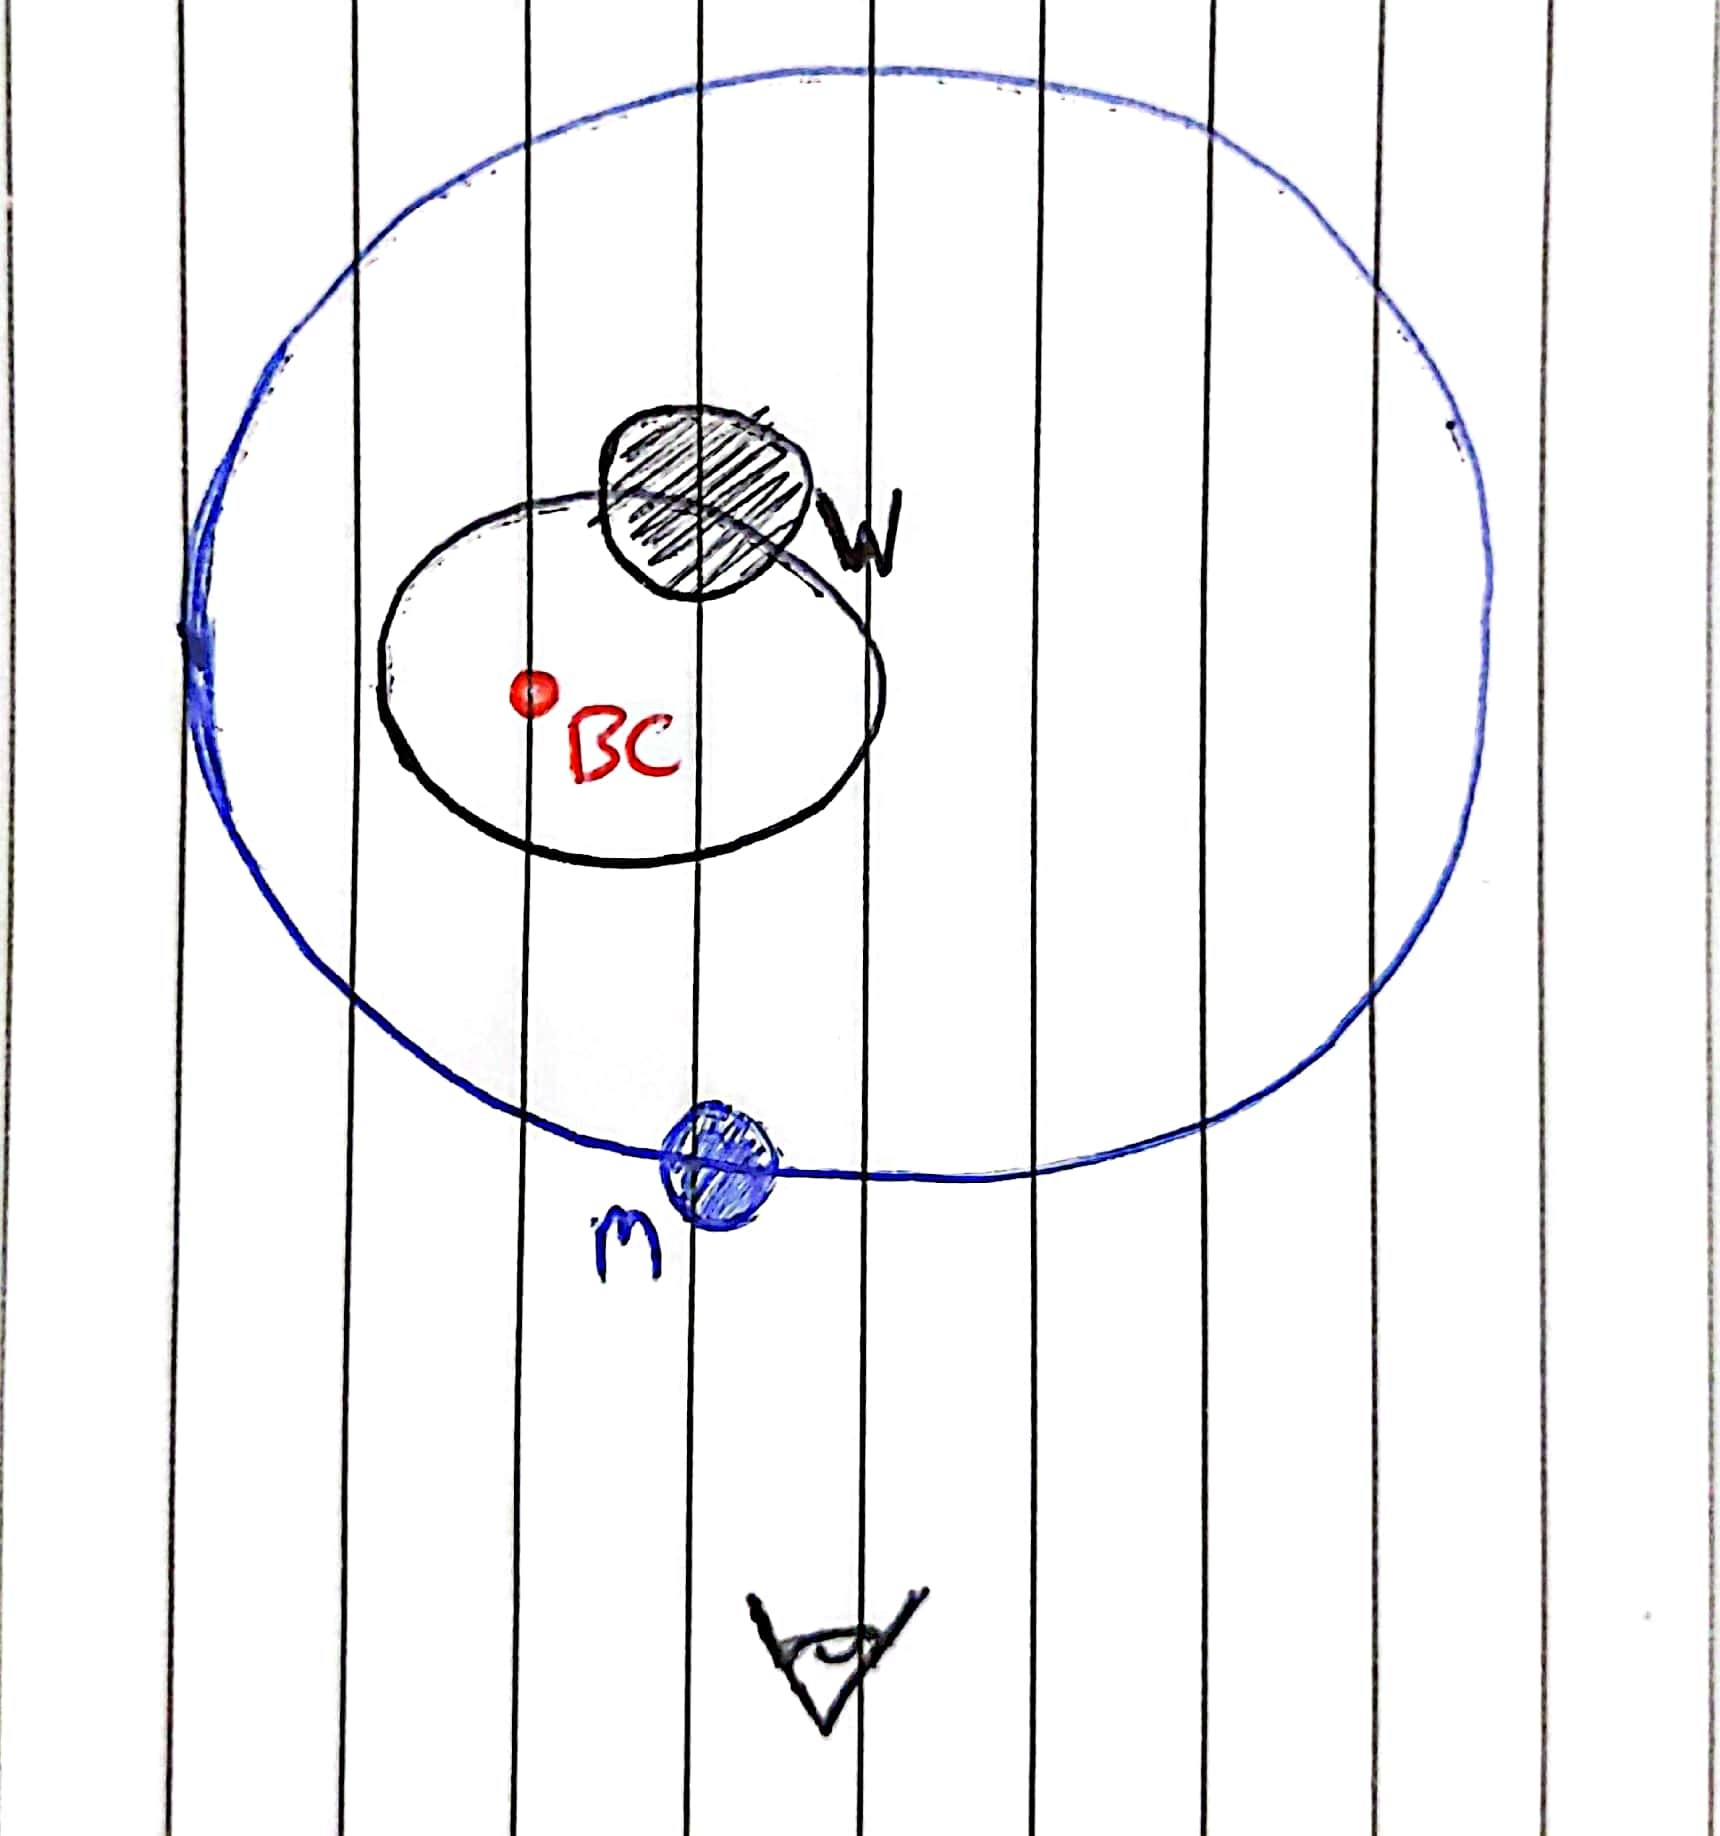
\includegraphics[width=0.5\columnwidth]{diagram.jpg}}
					\caption{\label{fig:diagram}A system diagram of NN Serpentis. The larger white dwarf (W) travels on the inner orbit whereas the smaller and dimmer red dwarf (M) travels on the outer orbit. They both orbit with the barycentre (BC) at their focus. The observer is marked at the bottom of the figure. It is visually clear how the red dwarf can eclipse the white dwarf.}
				\end{figure}	
		
	\section{Results and Analysis}
	
		\subsection{Messier 91}
		
			The angular size of M91 was plotted with a tolerance of 22 counts as an ellipse in red in figure \ref{fig:angSize}. An uncertainty on the tolerance was determined by increasing it until the ellipse was visually definitely inside the bounds of the galaxy and decreasing it until the ellipse was visually definitely outside the bounds of the galaxy. This uncertainty on the tolerance $\Delta T$ was determined to be $\pm 4 \,\text{counts}$. The upper limit on the apparent size was plotted in purple and the lower limit in orange. At a distance of $15\,\text{kpc}$, the apparent size of M91 was calculated to be $\left(21.8 \pm 4.3\right) \,\text{kpc}$ on the X axis and $\left(20.7 \pm 4.5\right) \,\text{kpc}$ on the Y axis. After adjusting for a position angle of $150^\circ$ and inclination of $36.9^\circ$ these increased to a physical size of $\left(54 \pm 11\right) \,\text{kpc}$ and $\left(51 \pm 11\right) \,\text{kpc}$ respectively. The Hyperleda catalogue of principle galaxies (2003)\cite{hyperleda} lists the angular size of M91 to be $5.37 \times 4.47\,\text{arcminutes}$ which, at the same distance as in our calculations corresponds to an apparent size of $\left(23.4 \pm 0.2\right) \,\text{kpc}$ by $\left(19.5 \pm 0.2\right) \,\text{kpc}$. These figures are within half of the range of uncertainty on our calculated values for the apparent size however this could become more accurate if this process was repeated on a larger dataset and if they were taken at longer exposures to reduce the signal-to-noise ratio.
			
			\begin{figure}
				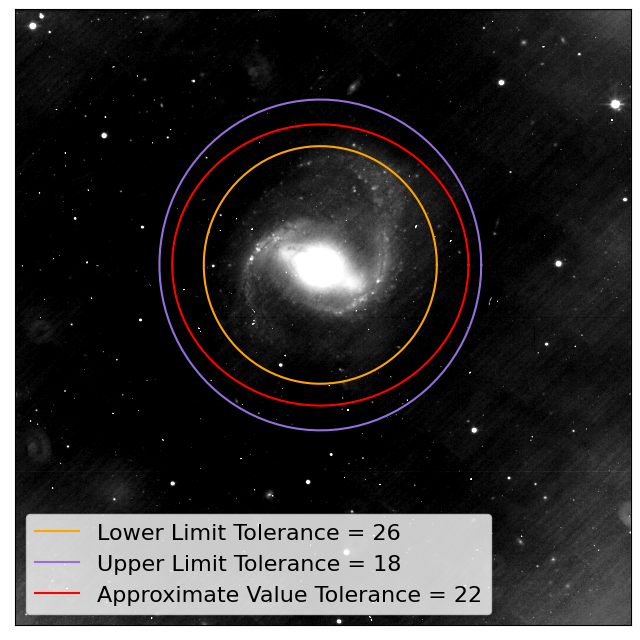
\includegraphics[width=\columnwidth]{angularSize.png}
				\caption{\label{fig:angSize} The reduced and combined image of Messier 91 with ellipses displaying the angular size. The red middle ellipse marks the calculated angular size with the baseline tolerance of 22 counts. The inner and outer ellipses mark the estimated bounds of uncertainty on the angular size. These were determined by changing the tolerance until the ellipse reached a position at which the angular size was either definitely larger (in the case of the outer bound) or definitely smaller (in the case of the inner bound) than the apparent angular size. This process of varying the tolerance to find appropriate bounds was done visually.}
			\end{figure}
			
		
		\subsection{NN Serpentis}
			The magnitude of NN Ser and the limiting magnitudes from when it was eclipsed were plotted against the time the images were taken, with the first image at time $t=0$. This created the lightcurve which is plotted in figure \ref{fig:lightcurve}. The uncertainty on these magnitudes is a combination of the uncertainty on the zeropoint, the standard deviation of the distribution of zeropoints, and the uncertainty on the photometry, equation \ref{eq:sigUncertainty}. It is important to note that the limiting magnitudes are simply an upper limit on what the magnitude of NN Ser could be and the actual eclipsed magnitude is unknown. To determine the duration of the eclipse, a gaussian was fitted to the dataset using least squares fitting. While this is somewhat non-physical, due to the limiting magnitude not representing actual data points for the lightcurve, it does still provide a good estimate on the duration of the eclipse by taking the width of four standard deviations. A width of four standard deviations on a gaussian distribution covers approximately 95\% of the area underneath the curve and therefore it is a good approximation of the eclipsed duration. The duration of the eclipse was determined to be $(11.1 \pm 1.2)\,\text{minutes}$. The uncertainty on this measurement comes from the uncertainty on the standard deviation fitting parameter of the least squares fit. This was determined by taking the square root of the diagonal elements of the covariance matrix. This was compared to reference measurements of previous eclipses by Parsons et al. (2010)\cite{times}. Although precise calculations of the duration of the eclipse aren't listed in their data, an estimate of an approximate value was determined graphically from their lightcurve to be $10.8 \,\text{minutes}$ which is within uncertainty of our calculated figure. From this lightcurve, a lower limit on the radio of the radii of the bodies can be determined. Using the following equation \ref{eq:depth} which relates the ratios of the radii to the depth of the lightcurve\cite{transit}:
			\begin{equation}
				R_t = R_\star \sqrt{\text{Depth}}
				\label{eq:depth}
			\end{equation}where the depth is a percentage depth of the lightcurve. Taking the minimum depth of a full eclipse to be the faintest point in figure \ref{fig:lightcurve}, the ratio of the masses was calculated to be at least greater than $0.7 \pm 0.3$. As this is just a limit, it doesn't tell us much. More images to fill the gaps in the light curve would help provide a better estimate. To better constrain the system images taken at a narrower field of view to focus on NN Ser and images taken with longer exposures to increase the signal-to-noise ratio should be taken.
			
			\begin{figure}
				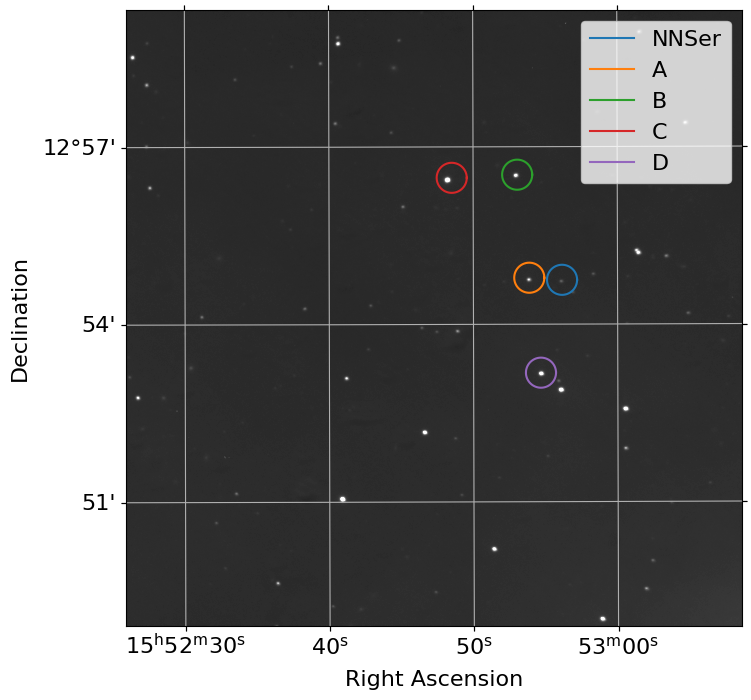
\includegraphics[width=\columnwidth]{rBandStars.png}
				\caption{\label{fig:rBandStars} An image of NN Serpentis. The reference stars used to calibrate the system to the r filter are circled to identify them.}
			\end{figure}	
			
			\begin{figure}
				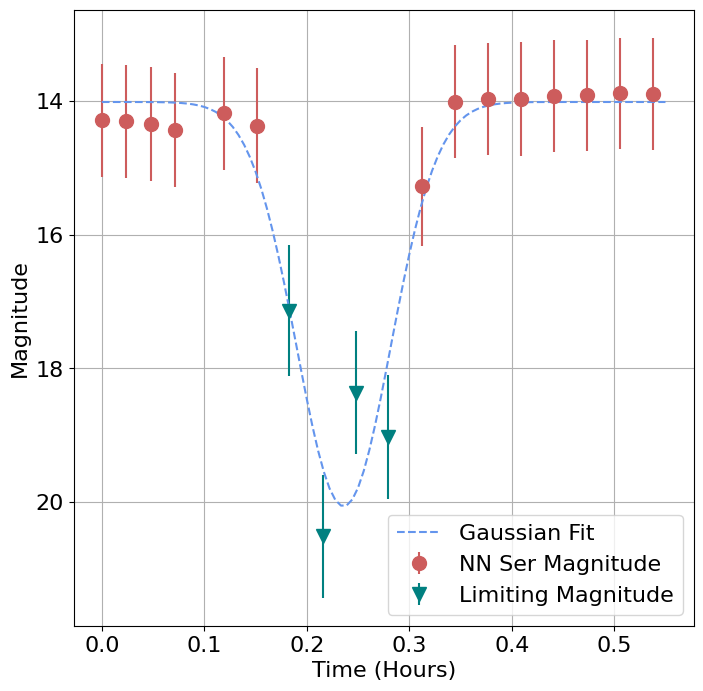
\includegraphics[width=\columnwidth]{lightcurve.png}
				\caption{\label{fig:lightcurve} Caption}
			\end{figure}

	\section{Conclusion}
		We calculated the apparent size of Messier 91 to be $\left(21.8 \pm 4.3\right) \,\text{kpc}$ $\times$ $\left(20.7 \pm 4.5\right) \,\text{kpc}$ which corresponds well to reference figures from Hyperleda\cite{hyperleda}. Adjusting for a position angle of $150^\circ$ and an inclination of $36.9^\circ$, the physical size of the galaxy was calculated to be $\left(54 \pm 11\right) \,\text{kpc}$ $\times$ $\left(51 \pm 11\right) \,\text{kpc}$. The lightcurve of NN Serpentis was plotted and the duration of the eclipse was determined to be $(11.1 \pm 1.2)\,\text{minutes}$ which is within uncertainty of that found in reference measurements\cite{times}. From this light curve, a lower limit on the ratio of the smaller mass to the larger mass of the two stars in NN Serpentis was calculated to be $0.7 \pm 0.3$.
		
	\newpage
	\bibliography{AstroAnalysis}% Produces the bibliography via BibTeX.
		
	\newpage
	\appendix
		
		
\end{document}

